\setcounter{MaxMatrixCols}{16}

\chapter{Теория}

\section{Матрица Адамара}

Сначала дадим определение марице Адамара.
\begin{Df}[Матрица Адамара]\normalfont\label{df:had_m}
    Назовем квадратную матрицу $H$ порядка $n$, составленную из чисел $1$ и $-1$, столбцы которой ортогональны, {\it матрицей Адамара}, если верно соотношение:
    \begin{equation}
        H H^T = n I_n,
    \end{equation}
    где $I_n$ -- это единичная матрица порядка $n$.
\end{Df}

\section{Алгоритм построения матриц Адамара}

Рассмотрим наивный алгоритм. Для наивного построения всех матриц Адамара заданного порядка $n$ достаточно перебрать все возможные кваратные матрицы порядка $n$, состоящие из чисел $1$ и $-1$, и найти те, которые удовлетворяют определению матрицы Адамара. Сложностная оценка у такого наивного метода будет $O(n^3 {2^{n^{2}}})$, так как проверка матрицы на Адамаровость требует $O(n^3)$ операций, а всего надо проверить $O({2^{n^{2}}})$ сгенерированных матриц. Такое число матриц обусловлено тем, что нужно для $n$ строк перебрать $2^n$ возможных значений. Такая сложность алгоритма является очень неоптимальной, так что рассмотрим более оптимальный алгоритм построения матриц Адамара.

Для ускорения наивного алгоритма можно использовать следующую идею: не перебирать все возможные квадратные матрицы, состоящие из $1$ и $-1$, а строить матрицу пошагово, строку за строкой, и при этом поддерживать множество $S(n)$ всех строк длины $n$ состоящих из $-1$ и $1$, которые ортогональнальны строкам из уже построенной части матрицы. Из множества $S(n)$ мы и будем брать следующую строку для построения матрицы Адамара. Если более формально, то этот алгоритм выглядит так:
\begin{enumerate}
    \item Проинициализировать первую строку матрицы $H$ единичной строкой, а множество $S(n)$ всеми строками, которые ортогональны начальной строке;
    \item На каждом последующем шаге построения матрицы $H$ берем следующую строку $h_i$ из $S(n)$ и прореживаем множество $S(n)$, оставляя только те, строки, которые ортогональны $h_i$;
    \item Если $S(n)$ опустело до того, как была достроена матрица $H$, то возвращаемся на шаг 2 и увеличиваем индекс $i$ на один;
    \item Если матрица $H$ достроена, то сохраняем $H$ и возвращаемся на шаг 2, увеличивая индекс $i$ на один, чтобы построить все оставшиеся матрицы порядка $n$.
\end{enumerate}

Из-за принципа работы алгоритма назовем его алгоритмом поиска матриц Адамара с возвратом.

Оценим сложность такого подхода. Для этого посчитаем, сколько раз мы обрабатываем одни и те же строки из множества $S(n)$. При фиксированной первой строке, состоящей из только из чисел $1$, для получения второй строки мы должны перебрать $C_n^\frac{n}{2} = \frac{n!}{\left(\frac{n}{2}\right)!\left(\frac{n}{2}\right)!}$ случаев, так как это число способов поставить $\frac{n}{2}$ нулей в строке из единиц длины $n$. Аналогично рассуждая, получим, что для построения третьей строки нам нужно рассмотреть $\left(C_\frac{n}{2}^\frac{n}{4}\right)^2$ случаев, так как это число способов расположить $\frac{n}{4}$ нулей в подпоследовательности из $\frac{n}{2}$ единиц, умноженное на число способов расположить $\frac{n}{4}$ единиц в подпоследовательности из $\frac{n}{2}$ нулей. Продолжая эту идею, получим, что необходимо рассмотреть $\frac{n!}{\left(\frac{n}{2}\right)!\left(\frac{n}{2}\right)!}\times\left(\frac{\frac{n}{2}!}{\left(\frac{n}{4}\right)!\left(\frac{n}{4}\right)!}\right)^2\times\cdots = n!$ строк, что хуже даже сложности наивного алгоритма. Однако, если зафиксировать первые три строки, то нужно будет перебрать $\left(\frac{n}{4}!\right)^4$ строк, что уже в разы лучше наивной сложности.

\section{Эквивалентность матриц Адамара по Холлу}

\begin{Df}[Эквивалентность матриц Адамара]\normalfont\label{df:had_eq}
    Две матрицы Адамара назовем {\it эквивалентными по Холлу}, если одна матрица может быть получена из другой при помощи следующих операций:
    \begin{enumerate}
        \item перестановка столбцов;
        \item перестановка строк;
        \item отрицание столбцов;
        \item отрицание строк.
    \end{enumerate}
    Эти операции будем называть операциями Холла. 
\end{Df}

Стоит заметить, что из любой матрицы Адамара существует $\left(n!\right)^2 2^{2n}$ способов построить другую матрицу, эквивалентную данной. Такое число переходов обусловлено тем, что сущствует $n!$ способов переставить строки и столбцы, а также существует $2^n$ способов отрицания строк и столбцов.

\section{Минимальная матрица Адамара}

Так как практический интерес представляют в основном только неэквивалентные матрицы из-за их различающихся свойств, то хочется в каждом классе эквивалентности выделить своего представителя, который был бы однозначно определим. Для этого введём понятие минимальной матрицы Адамара.

Для введения понятия минимальной матрицы Адамара нам понадобится сначала определить некую функцию, которая бы ставила в соответствие матрице размера $m \times n$ число так, что матрицы можно было бы упорядочить.

\begin{Df}\normalfont\label{df:bin_map}
    Пусть $A$ -- это двоичная матрица размера $m \times n$, тогда определим следующее отображение $\rho$ из множества двоичных матриц в множество целых чисел
    \begin{equation}
        \rho(A) \overset{\Delta}{=} \sum_{i = 1}^m \sum_{j = 1}^n \left[a_{ij} 2^{n(m-i)+(n-j)}\right],
    \end{equation}
    где $a_{ij}$ -- элемент матрицы $A$
\end{Df}

Данное отображение обладает следующими свойствами:
\begin{enumerate}
    \item Упорядоченность. Так как $\rho$ действует во множество целых чисел, то справедливо одно из следующих соотношений: $\rho(A) < \rho(B)$, $\rho(A) > \rho(B)$ или $\rho(A) = \rho(B)$ для любых двух двоичных матриц $A, B$ размера $m \times n$;
    \item Взаимная однозначность. $\rho(A) = \rho(B)$, тогда и только тогда, когда $A = B$ для любых двух двоичных матриц $A, B$ размера $m \times n$;
    \item Существование минимального элемента. Пусть $S$ -- множество двоичных матриц размера $m \times n$, тогда для любого подмножества $S_0$ множества $S$ существует матрица $M_0$, такая, что $\rho(M_0)$ -- минмимум для всех значений $\rho$ множества $S_0$, которую будем называть {\it минимальной матрицей} $S_0$. Более того, так как $\rho$ обладает свойством взаимной однозначности, то такая минимальная матрица единственна.
\end{enumerate}

\begin{Df}[Минимальная матрица Адамара]\normalfont\label{df:min_had}
    Пусть $H$ -- матрица Адамара, $H_{bin}$ -- двоичная матрица, полученная из матрицы $H$ заменой всех чисел $-1$ на $0$, тогда минимальная матрица $M$ двоичной матрицы $H_{bin}$ будет {\it минимальной матрицей класса эквивалентности}, содержащего $H_{bin}$. Матрицу $M$ будем называть минимальной матрицей Адамара.
\end{Df}

Стоит заметить, что при переходе от матрицы Адамара к ее двоичному представлению, следует заменить стандартное скалярное произведение на функцию исключающего или, чтобы поддержать свойство ортогональности строк и столбцов. Все остальные определения и свойства остаются в силе.

\section{Алгоритм поиска минимальной матрицы Адамара}
\label{mm_finder_th}

Воспользуемся алгоритмом построения минимальной матрицы, приведенным в статье \cite{park_song:he}. Для описания алгоритма вводится новая операция над матрицами Адамара.

\begin{Df}[Нормализация]\normalfont\label{df:norm}
    {\it Нормализация} -- это процесс преобразования двоичной матрицы $H$ с использованием только операций отрицания строк и операций отрицания столбцов в такое представление, что первая строка и первый столбец преобразованной матрицы состоят только из нулей.
\end{Df}

Процесс нормализации будем обозначать функцией $N$.

Алгоритм построения минимальной матрицы основывается на следующей теореме, которая определяет процесс построения минимальной матрицы в матричном виде. Приведем эту теорему без доказательства.

\begin{Th}\normalfont\label{th:mm_algo}
    \begin{enumerate}
        \item Минимальная матрица должна быть в нормализованной форме;
        \item Для двоичной матрицы $H$ и её минимальной матрицы $L$ существуют матрицы перестановок $P_r$ и $P_c$ такие, что
            \begin{equation}\label{eq:2}
                L = N(P_r H P_c);
            \end{equation}
        \item Если матрица $P_r$ и первый столбец матрицы $P_c$ известны, то оставшиеся столбцы матрицы $P_c$ могут быть определны из соотношения \ref{eq:2}.
    \end{enumerate}
\end{Th}

Основная идея алгоритма построения минимальной матрицы Адамара заключается в том, чтобы воспользоваться соотношением \ref{eq:2}. Для этого мы будем фиксировать первый столбец и первую строку матрицы Адамара, чтобы однозначно зафиксировать $N$, а после будем перебирать все возможные матрицы перестановок строк $P_r$, и для каждой такой матрицы $P_r$ будем подбирать матрицу перестановок $P_c$ так, чтобы значение $N(P_r H P_c)$ было минимальным. Главным же ускорением данного алгоритма является использование сортировки для подбора матрицы $P_c$. Опишем основные шаги алгоритма более подробно:
\begin{enumerate}
    \item Для входной двоичной матрицы $H_0$ размера $n \times n$ фиксируем первый столбец и первую строку, назовем полученную матрицу $H$;
    \item Применяем нормализацию $H = N(H)$;
    \item Пытаемся подобрать матрицы $P_r$, $P_c$, для этого запускаем функцию $CORE(H, A, r)$, где $r$ -- номер строки матрицы $P_r$, $A$ -- результат;
    \begin{enumerate}
        \item Среди строк с номером от $r+1$ до $n$ матрицы $H$ пытаемся найти такую, чтобы значение $\rho(H(r))$ было минимальным после перестановки этой строки с $r$-ой строкой для всех перестановок столбцов. Назовем такую строку $M$. Для этого после перестановки строки $M$ с $r$-ой строкой матрицы $H$ отсортируем полученную матрицу по столбцам, чтобы получить минимальное значение $\rho(H(r))$ для данной перестановки $P_r$ и к тому же определить для данной $P_r$ значение матрицы $P_c$ путем сортировки;
        \item Если значение $\rho(M)$ строки $M$, которая сейчас находится на позиции $r$, меньше, чем значение $\rho(A(r))$, то обновляем значение $A(r)$ на $M$. После вызываем $CORE(H, A, r+1)$;
    \end{enumerate}
    \item Обновляем результат -- минимальную матрицу и переходим к шагу 1.
\end{enumerate}

Таким образом, если использовать сортировку со сложностью $O(nlog(n))$, то итоговая сложностная оценка алгоритма будет выглядеть как $O((n!)n^2log(n))$. Такая сложность получается, потому что в алгоритме мы перебираем первый столбец и первую строку, фиксируя нормализацию $N$, что занимает $n^2$ операций, потом для каждой зафиксированной $N$ перебираем матрицы перестановок строк $P_r$ за $(n-1)!$ операций в худшем случае и для каждой $P_r$ ищем $P_c$ за сложность сортировки -- $O(nlog(n))$.

Однако стоит обратить внимание, что такая сложность -- это оценка сверху. В реальных условиях алгоритм работает гораздо быстрее за счёт того, что нам не преходится перебирать все $(n-1)!$ матриц $P_r$. Если внимательно посмотреть на шаги алгоритма, то можно заметить, что мы запускаем рекурсивную функцию $CORE$ только тогда, когда меняем $r$-ую строку со строкой $M$, а значит реальная сложность зависит от числа строк $M$ найденных на каждом шаге алгоритма, и таких строк в худшем случае было бы $(n-1)!$.

\section{Операции переключения}

Число классов эквивалентности по Холлу с ростом порядка растет очень быстро, например, известно, что для матриц Адамара порядка $16, 20, 24, 28, 32$ существует $5, 3, 60, 487, 13710027$ классов эквивалентности по Холлу, и нахождение новых классов является вычислительно сложной задачей. Из-за этого возникает потребность во введении нового более слабого понятия эквивалентности матриц Адамара, что позволит уменьшить число классов эквивалентности, а значит и упростит перечисление. Назовем такой тип эквивалентности Q-эквивалентностью.

Для введения нового понятия эквивалентности далее по тексту будут определены новые операции над матрицами Адамара, с помощью которых мы будем зачастую получать неэквивалентные по Холлу матрицы, при этом сохраняя свойства матрицы Адамара. Так как новое определение эквивалентности будет более слабым, то Q-неэквивалентные матрицы будут заведомо неэквивалентны по Холлу.

Основная идея новых операций над матрицами будет заключаться в том, чтобы искать в матрице некие подматрицы (блоки), отрицание которых бы сохраняло свойства матрицы Адамара, но производило новые неэквивалентные по Холлу матрицы. Для определения таких подматриц (блоков) дадим несколько вспомогательных определений.

\begin{Df}[Произведение Адамара]\normalfont\label{df:norm3}
    Пусть $H$ -- матрица Адамара размера $n$, тогда определим операцию {\it Адамарова произведения} двух строк $a$, $b$ как
    \begin{equation}
        (a_1, \cdots, a_n) \circ (b_1, \cdots, b_n) \overset{\Delta}{=} (a_1b_1, \cdots, a_nb_n).
    \end{equation}
\end{Df}

\begin{Df}[Три-нормализация]\normalfont\label{df:norm3}
    Пусть $H$ -- матрица Адамара размера $n$, тогда $H$ называется {\it три-нормализованной} для строк $H_i, H_j, H_k$, если $H_i \circ H_j \circ H_k = j_n$, где $j_n$ -- строка длины $n$, состоящая полностью из единиц.
\end{Df}

Классовая структура $(C_1, C_2, C_3, C_4)$ три-нормализованной матрицы Адамара $H$ размера $n$ представляет собой разбиение множества столбцов на четыре класса $C_i$, соответственно как $(H_{ic}, H_{jc}, H_{kc}) = (1, 1, 1), (-1, -1, 1), (-1, 1, -1)$ или $(1, -1, -1)$, где $H_{ic}$ -- множество элементов $i$-ой строки, участвующей в три-нормализации, принадлежащих классу $c$. Все четыре класса имеют длину $\frac{n}{4}$.

\begin{Df}\normalfont\label{df:norm3}
    Четвёрка строк $(i, j, k, l)$ матрицы Адамара $H$ размера $n$ называется {\it замкнутой}, если $H_i \circ H_j \circ H_k \circ H_l = \pm j_n$, где $j_n$ -- строка длины $n$, состоящая полностью из единиц.
\end{Df}

Из этого определения следует, что если матрица три-нормализована для любой тройки строк из замкнутой четвёрки, то четвертая строка обязана состоять только из $1$ или из $-1$.

Пример структуры матрицы с замкнутой четвёркой:\\
\begin{equation}\label{eq:mmod8}
    \begin{bmatrix}
        \bf{1} & \cdots & \bf{1} & - & \cdots & - & - & \cdots & - & 1 & \cdots & 1 \\
        \bf{1} & \cdots & \bf{1} & - & \cdots & - & 1 & \cdots & 1 & - & \cdots & - \\
        \bf{1} & \cdots & \bf{1} & 1 & \cdots & 1 & - & \cdots & - & - & \cdots & - \\
        \bf{1} & \cdots & \bf{1} & 1 & \cdots & 1 & 1 & \cdots & 1 & 1 & \cdots & 1 \\
        \multicolumn{3}{c}{$\vdots$} & \multicolumn{3}{c}{$\vdots$} & \multicolumn{3}{c}{$\vdots$} & \multicolumn{3}{c}{$\vdots$}
    \end{bmatrix}
\end{equation}

\begin{Df}[Операция переключения для матриц размера $n \equiv 0(mod 8)$]\normalfont\label{df:switch0}
    Пусть три-нормализованная матрица Адамара $H$ размера $n$ имеет замкнутую четвёрку строк, назовем эту четвёрку строк $Q$, и $(C_1, C_2, C_3, C_4)$ -- классовая структура матрицы, тогда {\it операцией переключения} называется отрицание всех элементов $h_{rc}$, таких что $r \in Q$ и $c \in C_i$ для любого $i \in \{1, 2, 3, 4\}$.
\end{Df}

Аналогичное определение можно ввести и для замкнутой четвёрки столбцов. 

Например, если применить операцию переключения к классу $C_1$ матрицы \ref{eq:mmod8}, то получится матрица вида:\\
\begin{equation}\label{eq:mmod0_switched}
    \begin{bmatrix}
        \boldsymbol{-} & \cdots & \boldsymbol{-} & - & \cdots & - & - & \cdots & - & 1 & \cdots & 1 \\
        \boldsymbol{-} & \cdots & \boldsymbol{-} & - & \cdots & - & 1 & \cdots & 1 & - & \cdots & - \\
        \boldsymbol{-} & \cdots & \boldsymbol{-} & 1 & \cdots & 1 & - & \cdots & - & - & \cdots & - \\
        \boldsymbol{-} & \cdots & \boldsymbol{-} & 1 & \cdots & 1 & 1 & \cdots & 1 & 1 & \cdots & 1 \\
        \multicolumn{3}{c}{$\vdots$} & \multicolumn{3}{c}{$\vdots$} & \multicolumn{3}{c}{$\vdots$} & \multicolumn{3}{c}{$\vdots$}
    \end{bmatrix}
\end{equation}

\begin{Df}[Операция переключения для матриц размера $n \equiv 4(mod 8)$]\normalfont\label{df:switch4}
    Пусть матрица Адамара $H$ размера $n$, где $n \equiv 4(mod8)$, представима в следующей форме:\\
    \begin{equation}\label{eq:m_4mod8}
        \begin{bmatrix}
            H_4 & F_1 & F_2 & F_3 & F_4 \\
            G_1 & A_{11} & A_{12} & A_{13} & A_{14} \\
            G_2 & A_{21} & A_{22} & A_{23} & A_{24} \\
            G_3 & A_{31} & A_{32} & A_{33} & A_{34} \\
            G_4 & A_{41} & A_{42} & A_{43} & A_{44}
        \end{bmatrix}
    \end{equation}
    где\\
    \begin{gather*}
        H_4 =
        \begin{bmatrix}
            1 & - & - & - \\
            - & 1 & - & - \\
            - & - & 1 & - \\
            - & - & - & 1
        \end{bmatrix}
        F_1 =
        \begin{bmatrix}
            1 & \cdots & 1 \\
            1 & \cdots & 1 \\
            1 & \cdots & 1 \\
            1 & \cdots & 1
        \end{bmatrix}
        F_2 =
        \begin{bmatrix}
            1 & \cdots & 1 \\
            - & \cdots & - \\
            1 & \cdots & 1 \\
            - & \cdots & -
        \end{bmatrix}
        \\
        F_3 = \begin{bmatrix}
            1 & \cdots & 1 \\
            - & \cdots & - \\
            - & \cdots & - \\
            1 & \cdots & 1
        \end{bmatrix}
        F_4 =
        \begin{bmatrix}
            - & \cdots & - \\
            - & \cdots & - \\
            1 & \cdots & 1 \\
            1 & \cdots & 1
        \end{bmatrix},
    \end{gather*}
    $G_1 = F_1^T, G_j = -F_j^T$ для $j \in \{2, 3, 4\}$ и $A_{ij}$ -- подматрицы такие, что сумма элементов каждого столбца и каждой строки равна $2$, когда $i=j$, и $0$, когда $i \neq j$. Тогда {\it операцией переключения} для такой матрицы назовем операцию замены $F_i$ на её отрицание и $G_i$ на её отрицание для любого $i = \{1, 2, 3, 4\}$.
\end{Df}

Стоит заметить, что согласно статье \cite{kimura:hs} матрицы $F_i$ и $G_j$ из определения \ref{df:switch4} образуют множество Холла.

Чтобы отличать операцию переключения для матрицы размера $n \equiv 0(mod8)$ от операции переключения для матрицы размера $n \equiv 4(mod8)$, будем называть первую операцию переключения как {\it операцию переключения замкнутой четвёрки}, а вторую операцию переключения как {\it операцию переключения множества Холла}.

\section{Q-эквивалентность матриц Адамара}

\begin{Df}[Q-эквивалентность]\normalfont\label{df:q_eq_df}
    Две матрицы Адамара $A$, $B$ размера $n$, где $n \equiv 0(mod8)$, называются {\it Q-эквивалентными}, если $B$ может быть получена из $A$ путем применения следующих операций:
    \begin{enumerate}
        \item отрицание столбцов;
        \item отрицание строк;
        \item операция переключения замкнутой четвёрки для строк;
        \item операция переключения замкнутой четвёрки для столбцов.
    \end{enumerate}
    Если $n \equiv 4(mod8)$, тогда матрицы $A$ и $B$ называются Q-эквивалентными, если $B$ может быть получена из $A$ путем применения следующих операций:
    \begin{enumerate}
        \item отрицание столбцов;
        \item отрицание строк;
        \item операция переключения для множества Холла.
    \end{enumerate}
\end{Df}

\section{Алгоритм поиска представителей классов Q-эквивалентности матриц Адамара}

Опишем алгоритм поиска представителей классов Q-эквивалентности матриц Адамара. Его главная идея будет заключаться в том, чтобы искать в исходной матрице подматрицы, которые имеют структуру представленную в \ref{eq:mmod8} и в \ref{eq:m_4mod8}. Искать данные подматрицы будем поэтапно, конструируя большую матрицую из меньших блоков. Выделив нужную структуру и совершив операцию переключения, будем добавлять новые полученные матрицы в список для обработки, чтобы обработать весь класс Q-эквивалентности целиком. Рассмотрим основные шаги алгоритма более подробно:
\begin{enumerate}
    \item Пусть дана матрица Адамара $H_0$ размера $n$, найдем минимальную матрицу матрицы $H_0$, назовем ее $M_0$.
    \item Проинициализируем список матриц, в котором будут содержаться все матрицы одного класса Q-эквивалентности, матрицей $M_0$. В данном списке будут именно минимальные матрицы, чтобы исключить повторную обработку двух эквивалентных по Холлу матриц.
    \item Пока список матриц не пуст, будем брать по одной матрице $H$.
    \begin{enumerate}
        \item Если $n \equiv 0(mod8)$:
        \begin{enumerate}
            \item Найдем в матрице $H$ замкнутые четвёрки, нужные для операций переключения;
            \item Производим операцию переключения для замкнутой четвёрки строк и столбцов;
            \item Находим минимальную матрицу новой полученной матрицы и складываем её в список матриц на обработку, если такой матрицы там еще не было;
        \end{enumerate}
        \item Если $n \equiv 4(mod8)$:
        \begin{enumerate}
            \item Найдем в матрице $H$ множества Холла, нужные для операций переключения;
            \item Производим операцию переключения для множества Холла;
            \item Находим минимальную матрицу новой полученной матрицы и складываем её в список матриц на обработку, если такой матрицы там еще не было.
        \end{enumerate}
    \end{enumerate}
\end{enumerate}

Дадим сложностную оценку такого алгоритма. В худшем случае на каждом шаге мы можем получить порядка $C_n^4$ новых матриц, так как столько возможных замкнутых четвёрок строк или множеств Холла в матрице размера $n$. Итого, учитывая, что алгоритм поиска минимальной матрицы имеет сложность в худшем случае $O((n!)n^2log(n))$, получаем итоговую сложность алгоритма: $O((n!)n^6log(n))$, так как для каждой новой матрицы мы ищем минимальную матрицу. Опять же, стоит обратить внимание, что это оценка сверху, и в реальности алгоритм работает в разы быстрее.

\chapter{Практическая часть}

% Алгоритмы в практической части будут представлены в псевдокоде, чтобы лучше передать основные моменты и тонкости реализации, не углубляясь в детали конкретного языка программирования.

% Реализацию основных частей программы можно будет найти в приложении к дипломной работе.

\section{Структура проекта}

Для реализации вышеперечисленных алгоритмов был выбран язык C++. Для сборки решения используется CMake.

Программу можно разделить на три составные части: функционал для работы со строками матрицы, реализацию двоичной матрицы и реализацию матрицы Адамара. Такая декомпозиция позволяет логически изолировать низкоуровневые части от высокоуровневых, что позволяет реализовывать сложные алгоритмы, используя более выразительный функционал, не задумываясь о деталях реализации.

Строка двоичной матрицы представлена отдельным классом, в котором определены необходимые методы для работы со строками. Данные внутри строки представляются целым 64-битным числом, это нужно по нескольким причинам. Первая причина заключается в том, чтобы основные функции над строками производить в битовых операциях, что более эффективно, так как они использую меньшее число процессорных инструкций, также такое представление позволяет эффективнее использовать кэш процессора. Вторая же причина в том, что это более эффективно по памяти, чем хранить данные в другом контейнере, например векторе. Стоит заметить, что такое представление подходит лишь для строк, чья длина не превосходит 64.

Двоичная матрица представляется вектором двоичных строк. В рамках данного класса реализованы такие операции как: отрицание строки, перестановка двух строк, перестановка столбцов, транспонирование матрицы, нормализация матрицы, а также сортировка столбцов матрицы.

Класс матрицы Адамара же представляет из себя расширение класса двоичной матрицы. В нем реализована обработка пользовательских данных, построение матриц Адамара, алгоритм поиска минимальной матрицы и алгоритм поиска представителей классов Q-эквивалентности.

Для первичной обработки входных данных, построения графиков по результатам работы программы и других вспомогательных функций использовался язык Python.

\section{Реализация алгоритма поиска минимальной матрицы Адамара}
\label{mm_finder_s}

Сначала реализуем алгоритм поиска минимальной матрицы, так как его можно использовать не только в алгоритме поиска представителей классов Q-эквивалентности матриц Адамара, но и в алгоритме построения матриц Адамара.

Логически реализация алгоритма будет разделена на две части: на основную функцию, которая будет фиксировать первую строку и первый столбец матрицы, и на рекурсивную функцию $CORE$, которая будет искать матрицы перестановок $P_r$ и $P_c$.

Основная функция будет принимать на вход матрицу Адамара размера $n \times n$. Реализацию функций перестановки строк, перестановки столбцов, нормализации и сортировки столбцов опустим, так как эти функции тривиальны.

\begin{figure}[H]
    \centering
    \begin{minipage}{\linewidth}
    \begin{lstlisting}[language=c++, tabsize=4, showspaces=false, basicstyle=\fontsize{9.5}{9.5}\selectfont, numbers=none]
    Matrix GetMinimalMatrix(const Matrix& m)
    {
        auto order = m.Order(); // порядок матрицы m
        auto result = m;
        result.Normalize();
        auto h = m;
        for (auto j = 0; j < order; ++j)
        {
            h.ColumnsSwap(0, j);    // фиксируем первый столбец
            for (auto i = 0; i < order; ++i)
            {
                h.RowsSwap(0, i);   // фиксируем первую строку
                h.Normalize();
                Core(result, h, 1, false);  // запускаем функцию по поиску минимальной матрицы
                h.RowsSwap(0, i);   // восстанавливаем матрицу
            }
            h = m;  // восстанавливаем матрицу
        }
        return result;
    }
    \end{lstlisting}
    \end{minipage}
    \caption{Алгоритм построения минимальной матрицы Адамара. Основная функция}
    \label{alg:mm_finder_main}
\end{figure}

Теперь приведем реализацию рекурсивной функции $CORE$ из алгоритма. 

\begin{figure}[H]
    \centering
    \begin{minipage}{\linewidth}
    \begin{lstlisting}[language=c++, tabsize=4, showspaces=false, basicstyle=\fontsize{9.5}{7.0}\selectfont, numbers=none]
    void Core(Matrix& result, Matrix& h, uint64_t r, bool flag)
    {
        auto order      = result.Order();
        if (r == order - 1) { // условие остановки рекурсии
            h.ColumnSort();
            if (flag || Rho(h[r]) < Rho(result[r])) { // если нашли меньшую строку
                result[r] = h[r];
            }
            return;
        }
    
        Row m{order, (1ULL << order) - 1}; // минимальная строка для $r$-ой позиции
        auto k = -1;
        std::vector<uint64_t> rowCandidates(order, 0);
        for (auto i = r; i < order; ++i) { // подбираем минимальную строку для $r$-ой позиции
            h.RowsSwap(i, r); // пытаемся найти такую строку, чтобы она была минимальной для r-ой позиции
            h.ColumnSort(); // ищем перестановку столбцов такую, чтобы матрица была как можно меньше
            if (Rho(h[r]) == Rho(m)) { // добавляем кандидата
                ++k;
                rowCandidates[k] = i;
            }
            if (Rho(h[r]) < Rho(m)) { // если получилось улучшить ответ, то обновляем кандидатов
                k = 0;
                rowCandidates[k] = i;
                m = h[r];
            }
            h.RowsSwap(i, r);
        }
    
        if (flag || Rho(m) < Rho(result[r])) { // если нашли меньшую строку
            result[r] = m; // обновляем строку в ответе
            h.RowsSwap(r, rowCandidates[0]);
            h.ColumnSort();
            Core(result, h, r + 1, true); // форсированно обновляем строки от r+1 результата
            h.RowsSwap(r, rowCandidates[0]);
            for (auto i = 1; i <= k; ++i) { // проверяем остальных кандидатов
                h.RowsSwap(r, rowCandidates[i]);
                h.ColumnSort();
                Core(result, h, r + 1, false);
                h.RowsSwap(r, rowCandidates[i]);
            }
        }
        if (!flag && m == result[r]) { // если мы уже имеем минимальную строку на r-ой позиции
            for (auto i = 0; i <= k; ++i) { // запускаем поиск минимальных строк для подматрицы
                h.RowsSwap(r, rowCandidates[i]);
                h.ColumnSort();
                Core(result, h, r + 1, false);
                h.RowsSwap(r, rowCandidates[i]);
            }
        }
    }
    \end{lstlisting}
    \end{minipage}
    \caption{Алгоритм построения минимальной матрицы Адамара. Рекурсивная функция CORE}
    \label{alg:mm_finder_core}
\end{figure}

Флаг $flag$ отвечает за форсированное (безусловное) изменение всех строк матрицы, начиная со строки с номером $r$. Это нужно для случая, когда мы на $i$-ую позицию в ответ вставили строку, которая в до этого в ответе была на $j$-ой позиции, причем $i < j$. То есть, если бы мы не изменяли эти строки, то получили бы в ответе две одинаковые строки на разных позициях.

Этот алгоритм можно ускорить. В основной функции алгоритма каждый раз ищется минимальная матрица для зафиксированной первой строки и для зафиксированного первого столбца. Если предположить, что мы имеем предпросчитанные минимальные матрицы Адамара, то можно заметить, что не обязательно перебирать все строки и столбцы, так как на какой-то итерации алгоритма мы могли уже построить минимальную матрицу и дальнейшая обработка бессмысленна.

Таким образом, перед поиском минимальной матрицы после фиксации первой строки и первого столбца, то есть перед вызовом функции $CORE$, можно вставить проверку на то, что мы уже нашли минимальную матрицу на данной итерации алгоритма, проверив, входит ли обрабатываемая матрица в число предпросчитанных матриц.

Приведем реализацию ускоренного алгоритма.

\begin{figure}[H]
    \centering
    \begin{minipage}{\linewidth}
    \begin{lstlisting}[language=c++, tabsize=4, showspaces=false, basicstyle=\fontsize{9.5}{7.0}\selectfont, numbers=none]
    Matrix GetMinimalMatrix(const Matrix& m, const std::unordered_set<std::string>& memo)
    {
        auto order = m.Order(); // порядок матрицы m
        auto result = m;
        result.Normalize();
        auto h = m;
    
        for (auto j = 0; j < order; ++j)
        {
            h.ColumnsSwap(0, j);    // фиксируем первый столбец
            for (auto i = 0; i < order; ++i)
            {
                h.RowsSwap(0, i);   // фиксируем первую строку
                h.Normalize();
                // проверка на то, достигли ли мы досрочно минимальной матрицы
                if (memo.count(result.ToString()))
                {
                    return result;
                }
                Core(result, h, 1, false);  // запускаем функцию по поиску минимальной матрицы
                h.RowsSwap(0, i);   // восстанавливаем матрицу
            }
            h = m;  // восстанавливаем матрицу
        }
    
        return result;
    }
    \end{lstlisting}
    \end{minipage}
    \caption{Алгоритм построения минимальной матрицы Адамара. Ускоренная версия}
    \label{alg:mm_finder_main_acc}
\end{figure}

Список предпросчитанных минимальных матриц представлен в виде хэш-таблицы, чтобы быстро искать вхождение матрицы в список. Сама матрица в хэш-таблице представлена в виде строки.

\section{Реализация алгоритма построения матриц Адамара}
\label{builder_s}

Функционал для генерации матриц Адамара будет реализован в виде отдельного класса.

\begin{figure}[H]
    \centering
    \begin{minipage}{\linewidth}
    \begin{lstlisting}[language=c++, tabsize=4, showspaces=false, basicstyle=\fontsize{9.5}{9.5}\selectfont, numbers=none]
    class Bucket
    {
    public:
        // Параметр order -- порядок матрицы
        explicit Bucket(uint64_t order, Mode mode);
        // Метод для генерации матриц Адамара
        void GenerateMatrix();
        // Метод для получения сгенерированных матриц
        const std::vector<Matrix>& GetFoundMatrices() const;
        ~Bucket() = default;
    
    private:
        using BucketContext = std::pair<std::deque<Row>, uint64_t>;
    
    private:
        // Просеить множество строк, оставив только те строки, что ортогональны строке row
        std::deque<Row> ReduceBucket(const Row& row, const std::deque<Row>& vec);
        // Просеить начальную корзину по базису из трех строк
        std::deque<Row> ReduceInitBucket(uint64_t maxVal);
    
    private:
        uint64_t                        m_order;
        // Частично построенная матрица Адамара
        Matrix                          m_completedRows;
        // Контекст построения матриц
        std::deque<BucketContext>       m_bucketHistory;
        // Найденные матрицы
        std::vector<Matrix>             m_foundMatrices;
        ThreadSafeSet<std::string>      m_UniqueMatricesSet;
    };
    \end{lstlisting}
    \end{minipage}
    \caption{Объявление класса для генерации матриц Адамара}
    \label{alg:builder_definition}
\end{figure}

Основной цикл алгоритма построения будет реализован в методе $GenerateMatrix$. Для его работы нам понадобятся вспомогательные методы $ReduceBucket$ и $ReduceInitBucket$. В методе $ReduceBucket$ мы будем просеивать множество строк, оставляя в нем только те строки, которые ортогональны переданной строке, а в методе $ReduceInitBucket$ будем задавать начальное множество строк -- то есть множество строк, ортогональных трём первым строкам матрицы Адамара. Реализация этих функций очевидна, поэтому не будем её здесь приводить.

Приведем реализацию метода $GenerateMatrix$, в котором будет находиться основной цикл алгоритма построения матриц Адамара.

\begin{figure}[H]
    \centering
    \begin{minipage}{\linewidth}
    \begin{lstlisting}[language=c++, tabsize=4, showspaces=false, basicstyle=\fontsize{9.5}{9.5}\selectfont, numbers=none]
    void Bucket::GenerateMatrix()
    {
        // пока не израсходовали все множество строк
        while (m_bucketHistory.size() != 0) {
            Row   nextRow;
            auto& [bucket, chosen] = m_bucketHistory.back();// берём ближайший контекст
            nextRow = bucket[chosen]; // выбираем следующую строку в матрице адамара
            ++chosen; // сдвигаем начальную строку в множестве
            // если множество опустело, то есть мы не смогли найти следующую строку
            if (nextRow.Count() == 0) {
                // бэктрекинг
                m_completedRows.PopBack();
                m_bucketHistory.pop_back();
                continue;
            }
            // просеиваем множество строк так, чтобы в нем остались только те строки,
            // которые ортогональны заданной
            auto reduced = ReduceBucket(nextRow, bucket);
            // достраиваем матрицу
            m_completedRows.PushBack(nextRow);
            // обновляем контекст, добавляя в него просеенное множество
            m_bucketHistory.push_back(BucketContext{reduced, 0});
            // если нашли матрицу, то сохраняем ее минимальное представление в set
            if (m_completedRows.Size() == m_order) {
                auto minMatrix = GetMinimalMatrix(m_completedRows,m_UniqueMatricesSet);
                if (!m_UniqueMatricesSet.count(minMatrix.ToString())) {
                    m_UniqueMatricesSet.insert(minMatrix.ToString());
                }
                // бэктрекинг
                m_completedRows.PopBack();
                m_bucketHistory.pop_back();
            }
        }
    }
    \end{lstlisting}
    \end{minipage}
    \caption{Алгоритм построения минимальной матрицы Адамара. Основной цикл}
    \label{alg:builder_main}
\end{figure}

Множество строк-кандидатов для построения матрицы Адамара будем представлять как упорядоченный контейнер. Стоит заметить, что в процессе построения матрицы, множество уменьшается, и так как мы хотим построить все матрицы данного размера с точностью до операций Холла, то необходимо поддерживать некий контекст, чтобы понимать, какие строки множества мы уже обработали, а какие ещё не обработали. Контекст будет представлен списком пар из упорядоченного контейнера и номера строки, на которой остановилась обработка на предыдущем этапе. Упорядоченный контейнер в данном случае будет играть роль множества строк-кандидатов для вставки на следующую позицию матрицы Адамара.

Сгенерировав очередную матрицу, будем хранить её минимальное представление в хэш-таблице. Это сделано для того, чтобы на выходе получать уникальные неэквивалентные по Холлу матрицы.

\section{Реализация алгоритма поиска представителей классов Q-эквивалентности матриц Адамара}

Алгоритм генерации новой матрицы при помощи операции переключения логически можно разделить на две основные части -- на поиск подматриц матрицы Адамара, описанных в теоритической части, и на получение новых матриц Адамара, применяя операцию переключения.

Поиск подматриц заключается в том, чтобы найти в матрице Адамара замкнутые четвёрки или множества Холла и выделить среди них один из четырёх классов согласно определению \ref{df:switch0} для замкнутой четвёрки или одну из четырёх пар подматриц согласно определению \ref{df:switch4} для множества Холла. В статье \cite{orrick:so} сказано, что класс эквивалентности матрицы Адамара, полученной переключением, не зависит от того, какой из четырёх классов или какую из четырёх пар мы выбираем для отрицания. Поэтому будем искать подматрицы, принадлежащие классу $C_1$ из определения \ref{df:switch0}, или подматрицы, принадлежащие паре $G_1, F_1$ из определения \ref{df:switch4}. Для краткости назовём такие подматрицы {\it подматрицами переключения}.

% подматрицы переключения
% матричные структуры

Подматрицы переключения будем строить из непересекающихся блоков размера $4 \times 4$, так как исходя из вышеупомянутых определений, подматрицы переключения будут иметь размер $4 \times \frac{k}{4}$ или $\frac{k}{4} \times 4$, где $k = n - n(mod8)$.

Искать блоки будем следующим образом:
\begin{enumerate}
    \item Зафиксируем четвёрку строк;
    \item Будем перебирать четвёрки столбцов для данной четвёрки строк так, чтобы на их пересечении образовалась подматрица $4 \times 4$, то есть блок;
    \item Если блок можно привести к матрице, состоящей полностью из единиц, используя операции Холла, то сохраним этот блок;
    \item Продолжим перебирать четвёрки столбцов, исключая четвёрки, в которых присутствуют использованные позиции, чтобы гарантировать, что блоки не пересекаются.
\end{enumerate}

Данный алгоритм также следует повторить для транспонированной матрицы Адамара, чтобы найти замкнутые четвёрки столбцов.

Приведём реализацию метода поиска блоков. Метод принимает на вход матрицу Адамара, вектор возможных позиций всех четвёрок строк и столбцов и также структуру, в которую будут сохраняться блоки. Блок будет сохраняться в виде позиций строк и столбцов, которые его образуют, а также информации о том, какие строки и столбцы надо подвергнуть отрицанию, чтобы получить блок, состоящий из единиц. Эта информация понадобится нам в будущем, когда мы будем конкатенировать блоки в подматрицы размера $4 \times \frac{k}{4}$ или $\frac{k}{4} \times 4$, где $k = n - n(mod8)$.
\begin{figure}[H]
    \centering
    \begin{minipage}{\linewidth}
    \begin{lstlisting}[language=c++, tabsize=4, showspaces=false, basicstyle=\fontsize{9.5}{11.5}\selectfont, numbers=none]
    void Classifier::FindBlocks(const Matrix&                             matrix,
                                const std::vector<std::vector<uint64_t>>& rowsPositions,
                                const std::vector<std::vector<uint64_t>>& colsPositions,
                                MatrixMemoStruct&                         memo) const
    {
        // фиксируем четвёрку строк
        for (const auto& nextRowsPos: rowsPositions) {
            // инициализируем множество использованных столбцов
            std::unordered_set<uint64_t> used;
            std::vector<Classifier::BlockInfo> tmpMemo;
    
            // фиксируем блок
            for (const auto& nextColsPos: colsPositions) {
                uint64_t rowsToNegateMask;
                uint64_t colsToNegateMask;
    
                // проверяем, есть ли среди столбцов уже использованные
                bool isUsed = false;
                for (auto pos: nextColsPos) {
                    if (used.count(pos)) {
                        isUsed = true;
                    }
                }
                // если есть использованные столбцы, то не рассматриваем такой блок
                if (isUsed) {
                    continue;
                }
                // если блок приводим к матрице, состоящей из единиц
                if (CheckOneMatrix(matrix, nextRowsPos, nextColsPos, rowsToNegateMask, colsToNegateMask)) {
                    auto rowMask = GetMask(nextRowsPos);
                    auto colMask = GetMask(nextColsPos);
                    // сохраняем блок
                    tmpMemo.emplace_back(rowMask, colMask, rowsToNegateMask, colsToNegateMask, nextRowsPos, nextColsPos);
                    used.insert(nextColsPos.begin(), nextColsPos.end());
                }
            }
            // сохраняем блок
            if (tmpMemo.size() != 0) {
                auto key = MakeMemoKey(nextRowsPos);
                memo.insert({key, std::move(tmpMemo)});
            }
        }
    }
    \end{lstlisting}
    \end{minipage}
    \caption{Функция для поиска блоков в матрице Адамара}
    \label{alg:blocks_finder}
\end{figure}

Когда все блоки получены, можно перейти к построению подматриц переключения. Для этого будем конкатенировать блоки, находящиеся на одной и той же четвёрке строк или столбцов. Для корректного построения подматриц переключения стоит учитывать совместимость блоков, то есть что они принадлежат одному классу.

Построив подматрицу переключения, необходимо применить к нему операцию отрицания, чтобы получить новую матрицу Адамара. Строго говоря, при данном подходе построения подматриц переключения мы не учитываем остальную структуру матрицы, а лишь пытаемся найти класс $C_1$ или подматрицы $G_1$ и $F_1$, так что нет гарантии, что структура матрицы Адамара соответствует определениям \ref{df:switch0} и \ref{df:switch4}. Поэтому, получив новую матрицу, следует проверить, что она удовлетворяет определению матрицы Адамара.

После, сгенерировав новую матрицу, нужно построить для нее минимальную матрицу и сохранить её в очередь для обработки. Как только очередь опустеет -- все матрицы для данного класса Q-экивалентности будут найдены.

Приведём реализацию главного цикла основного метода алгоритма поиска представителей классов Q-эквивалентности для случая $n \equiv 0(mod8)$. Метод принимает на вход вектор матриц Адамара и вычисляет, к какому классу Q-эквивалентности они принадлежат.

\begin{figure}[H]
    \centering
    \begin{minipage}{\linewidth}
    \begin{lstlisting}[language=c++, tabsize=2, showspaces=false, basicstyle=\fontsize{8}{9}\selectfont, numbers=none]
    std::vector<uint64_t> Classifier::Classify(const std::vector<Matrix>& matrices) const
    {
        std::vector<uint64_t> result;
        auto countOfBlocks     = m_order / 16;
        // генерируем всевозможные позиции для блоков
        auto blockPositions    = GetAllPos(4, 0, m_order);
        for (const auto& startMatrix: matrices) {
            // инициализация очереди обработки
            auto minStartMatrix = GetMinimalMatrix(startMatrix);
            auto strStartMatrix = minStartMatrix.ToString();
            std::vector<Matrix> candidates;
            candidates.push_back(minStartMatrix);
            // пока очередь не опустела
            for (auto next = 0; next < candidates.size(); ++next) {
                auto matrix = candidates[next];
                // структура для хранения блоков
                MemoContext blocksMemo;
                // ищем блоки
                FindBlocks(matrix, blockPositions, blockPositions, blocksMemo.rowBlocksMemo);
                FindBlocks(matrix.GetTransposed(), blockPositions, blockPositions, blocksMemo.colBlocksMemo);
                if (m_order % 8 == 0) {
                    // случай применения операции переключения для строк
                    for (const auto& [rowsKey, quadruple]: blocksMemo.rowBlocksMemo) {
                        std::vector<uint64_t> indexes(this->m_order / 16, 0);
                        std::vector<uint64_t> endPerIndex(this->m_order / 16, quadruple.size());
                        std::vector<Matrix>   newMatrices;
                        // из блоков 4x4 строим блоки размера 4x(n/4) и применяем операцию переключения
                        RecursiveMatrixBuild(indexes, endPerIndex, 0, 0, matrix, quadruple, newMatrices, false);
                        for (const auto& newMatrix: newMatrices) {
                            // проверяем, что полученная матрица соотв-ет определению матрицы Адамара
                            if (!newMatrix.IsHadamard()) {
                                continue;
                            }
                            // ищем минимальную матрицу для построенной новой матрицы
                            auto minMatrix = GetMinimalMatrix(newMatrix);
                            auto strMatrix = minMatrix.ToString();
                            // если такой матрицы еще не встречалось
                            if (!this->m_cachedQClasses.back().count(strMatrix)) {
                                // то добавляем ее в очередь обработки
                                this->m_cachedQClasses.back().insert(strMatrix);
                                candidates.push_back(minMatrix);
                            }
                        }
                    }
                    // аналогично случай применения операции переключения для столбцов
                    // ...
                } else {
                    // ...
                }
            }
        }
        return result;
    }
    \end{lstlisting}
    \end{minipage}
    \caption{Основная функция алгоритма поиска представителей классов Q-эквивалентности для случая $n \equiv 0(mod8)$}
    \label{alg:q_finder}
\end{figure}

Итого, весь алгоритм можно в общих чертах представить в виде следующей схемы.

\begin{figure}[H]
    \centering
    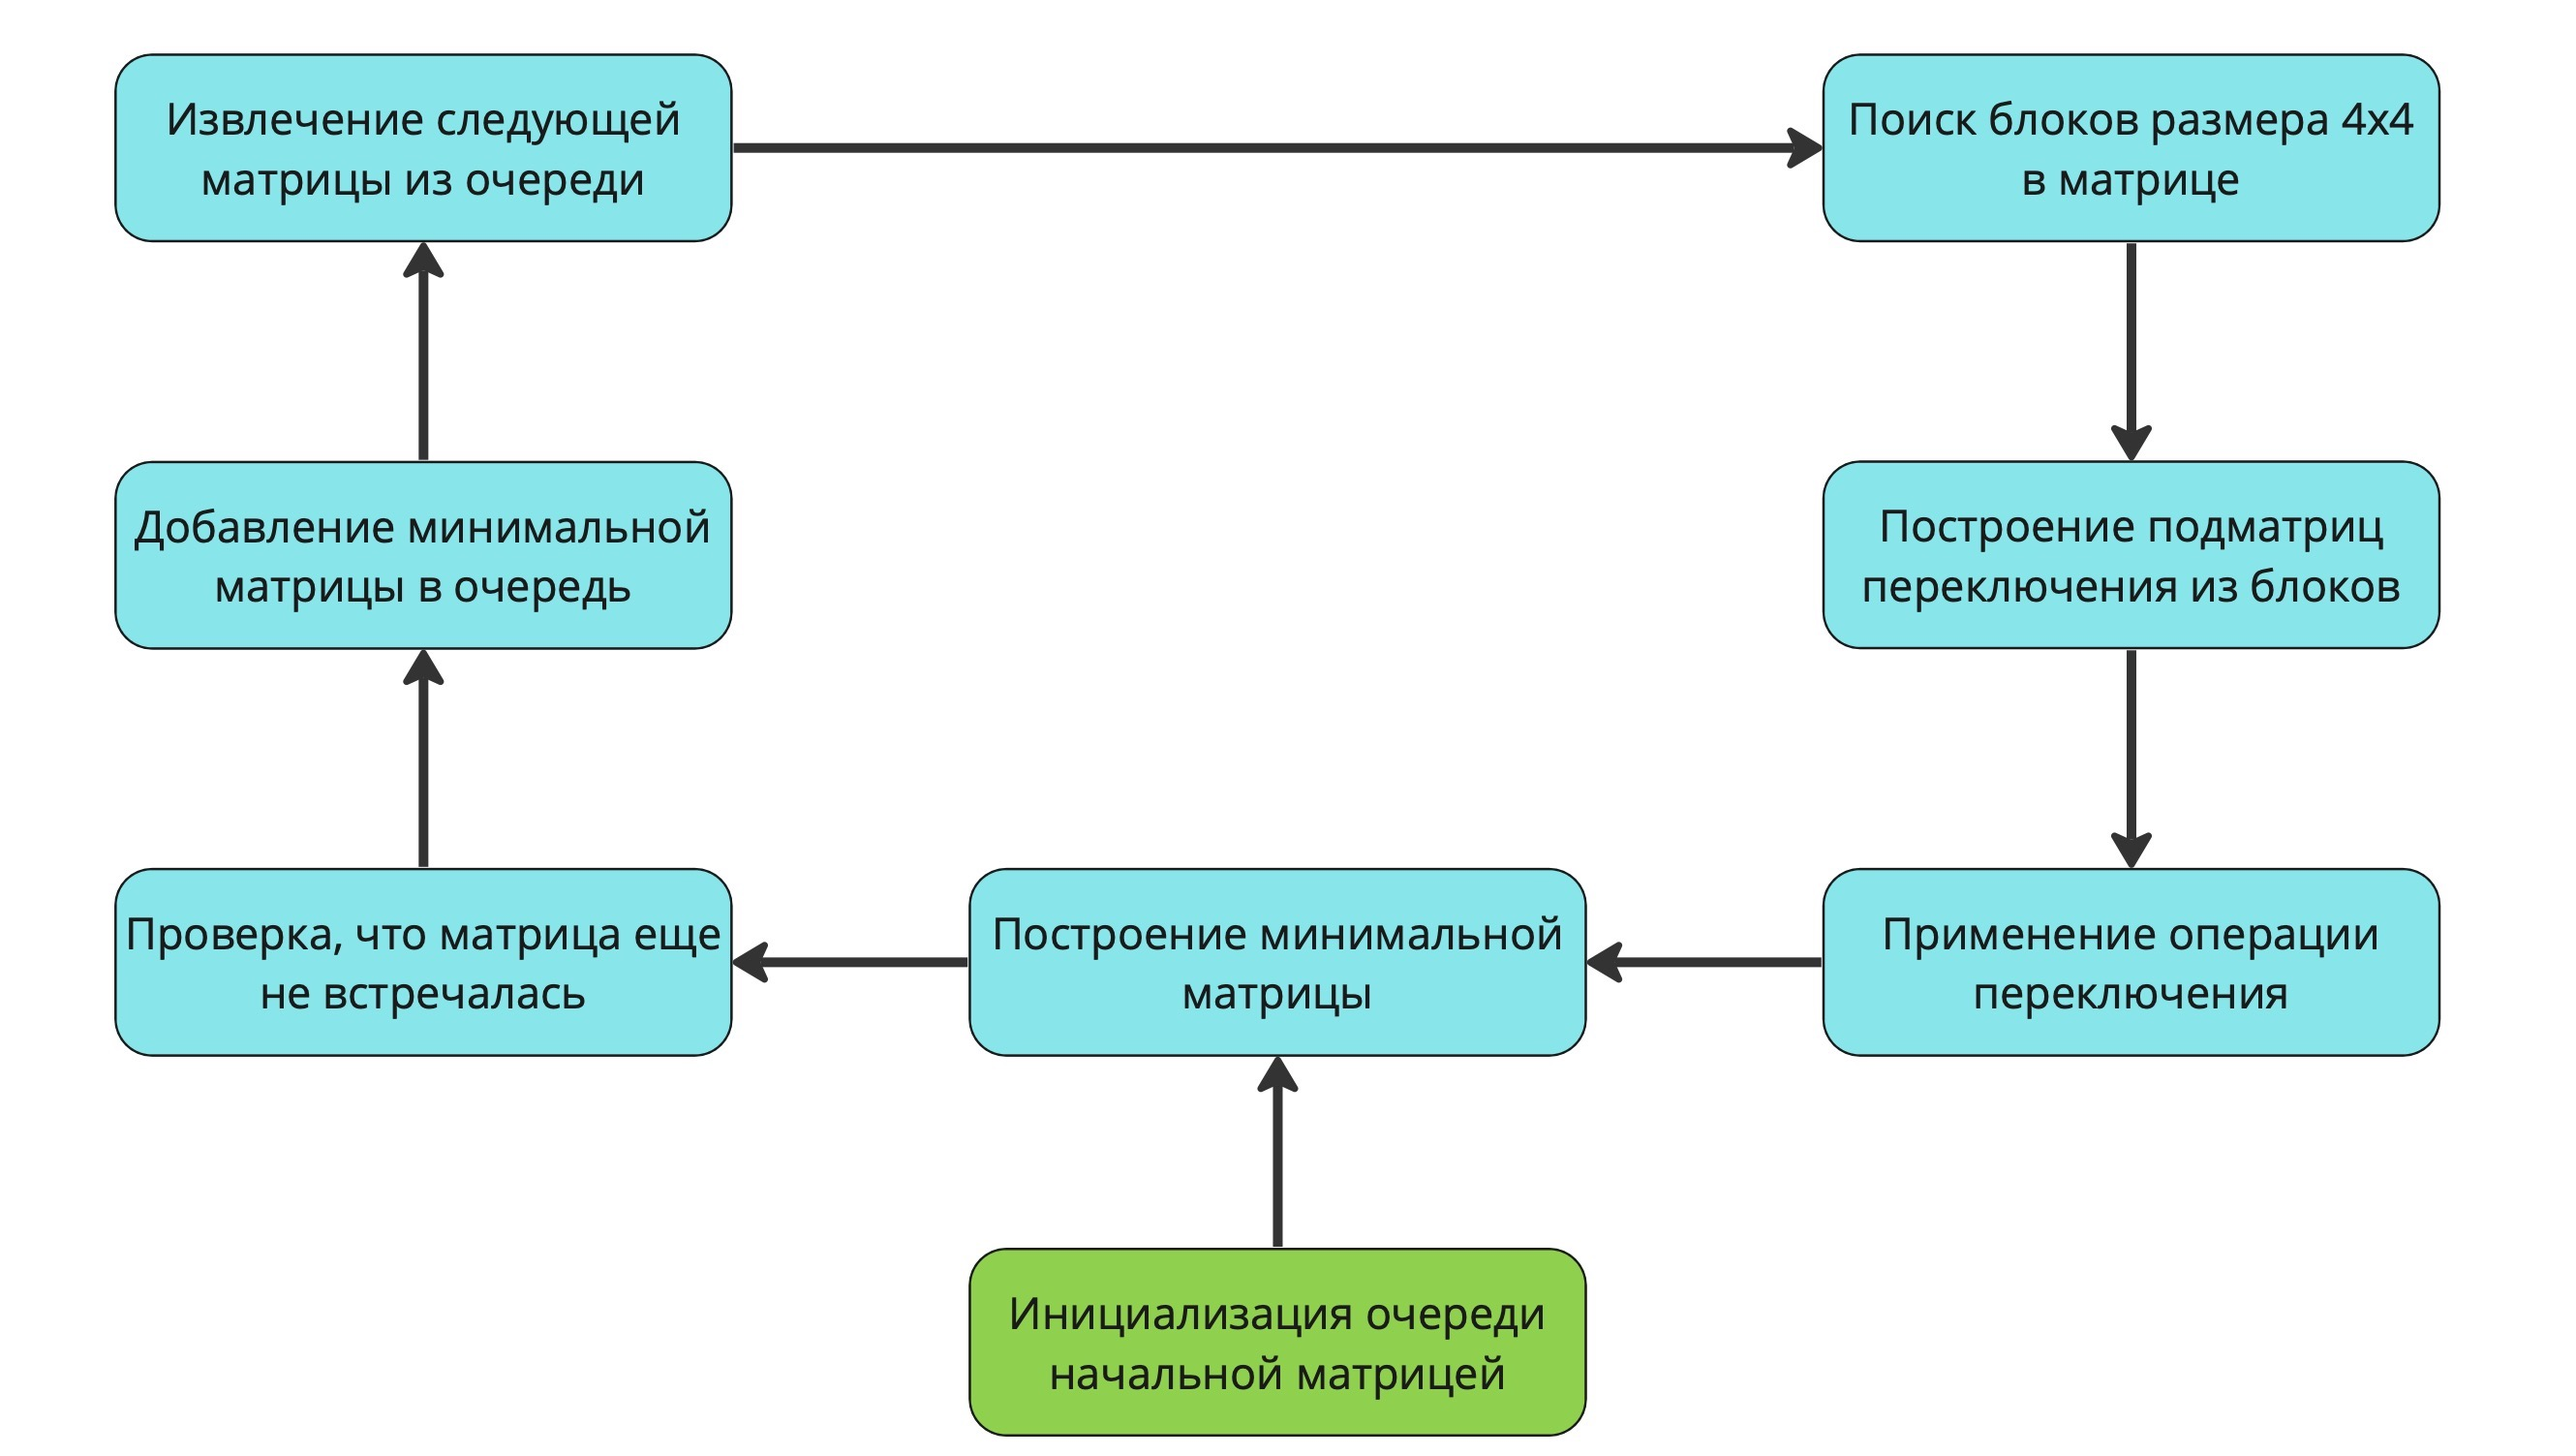
\includegraphics[scale=0.17]{res/img/plot_algo.jpg}
    \caption{Схема работы алгоритма поиска представителей классов Q-эквивалентности}
    \label{fig:algo}
\end{figure}

\section{Оптимизация алгоритма поиска представителей классов Q-эквивалентности матриц Адамара}

Самой вычислительно сложной операцией данного алгоритма является построение минимальной матрицы.

Чтобы ускорить этот процесс, воспользуемся эвристикой из пункта \ref{mm_finder_s}, то есть предпросчитаем и сохраним минимальные матрицы размера $n$ для предствителей всех классов эквивалентности по Холлу. Эти матрицы можно получить, сгенерировав при помощи алгоритма из пункта \ref{builder_s}, или взяв с ресурса \cite{sloane:lhm}. Для краткости будем называть такое ускорение использованием {\it контекста}.

Второй идеей для ускорения будет распараллеливание процесса поиска минимальной матрицы.

Класс Q-эквивалентности матрицы Адамара можно представить в виде графа, в котором вершинами будут матрицы, а рёбрами будут операции переключения и построения минимальной матрицы. Поиск всех неэквивалентных по Холлу матриц, которые содержатся в одном классе Q-эквивалентности, можно представить как поиск в ширину для графа. Таким образом, операции построения минимальной матрицы в рамках одного фронта волны поиска в ширину можно запускать параллельно, так как они независимы.

\begin{figure}[h]
    \centering
    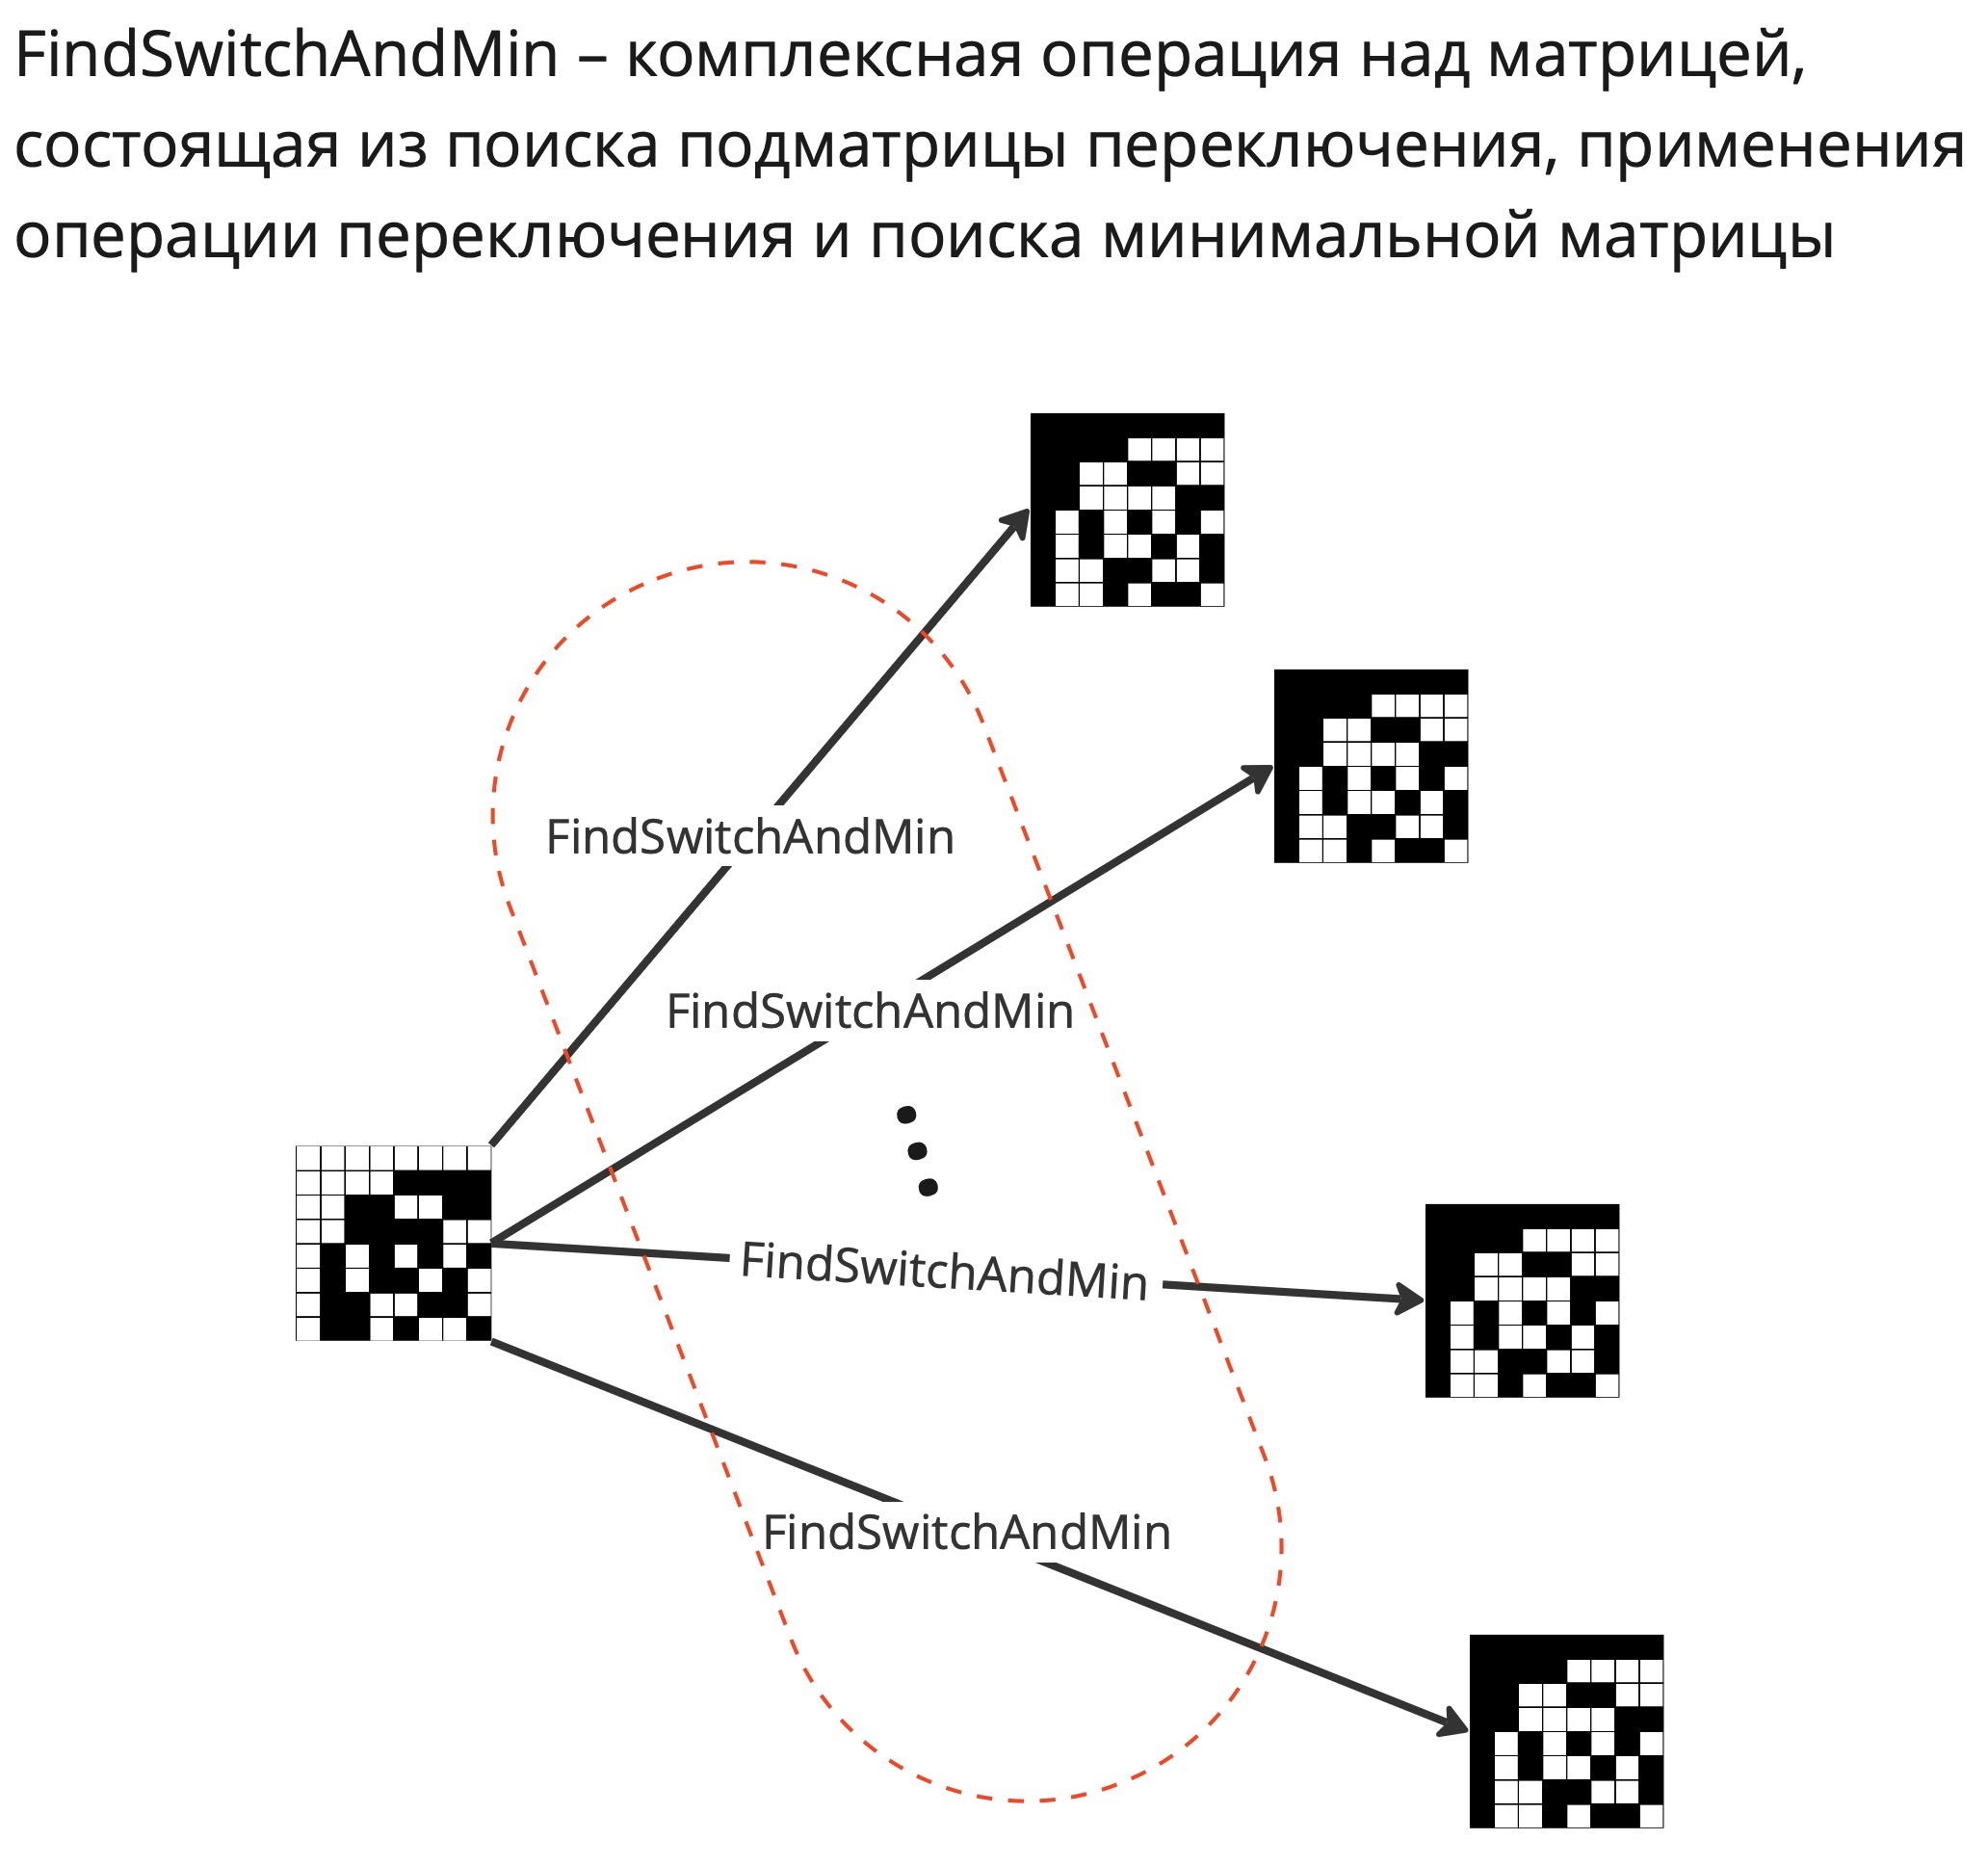
\includegraphics[scale=0.18]{res/img/graph.jpg}
    \caption{Частичный граф класса Q-эквивалентности}
    \label{fig:graph}
\end{figure}

На рисунке \ref{fig:graph} представлена часть графа класса Q-эквивалентности, где матрицами Адамара 8-го порядка обозначаются Q-неэквивалентные матрицы Адамара произвольного порядка, а красным пунктиром обозначены операции, которые могут быть запущены параллельно.

Для реализации данных ускорений нам потребуется поддерживать thread-safe множество предпросчитанных минимальных матриц. Для обеспечения thread-safety напишем обертку над стандартным unordered\_set из C++, а также защитим при помощи мьютекса очередь обработки матриц. Каждую операцию переключения вместе с последующим поиском минимальной матрицы будем воспринимать как отдельную задачу, которую будем складывать в thread pool. Синхронизировать потоки будем в конце каждого фронта волны поиска в ширину.

\section{Методика проведения измерений}

Основным параметром сравнения различных версий алгоритмов будет время работы программы. Будем сравнивать время работы для различных порядков входных матриц Адамара, это поможет понять динамику увеличения времени работы от увеличения порядка матрицы.

Производить измерения будем на виртуальной машине со следующими характеристиками: 8 процессоров Intel Xeon E3-12xx v2 (Ivy Bridge) с архитектурой x86\_64, 32 ГБ оперативной памяти.

Для тестирования многопоточной реализации использовалось 7 потоков.

\section{Результаты}

В качестве теста на корректность работы программы найдем число классов Q-эквивалентности для матриц порядка $16, 20, 24, 28$.

Программа получает на вход файл, в котором перечислены представители всех классов эквивалентности по Холлу указанных выше порядков. Результатом работы должен быть вывод о том, какие из переданных матриц в рамках одного порядка пренадлежат какому классу. Для порядков выше $28$-го число классов эквивалентности по Холлу исчисляется миллионами, поэтому представленная программа не сможет в разумное время решить задачу классификации, так что в рамках данной дипломной работы ограничимся $28$-м порядком.

Будем проверять три вариации алгоритма поиска представителей классов Q-эквивалентности матриц Адамара: вариант без оптимизаций, вариант с использованием предпросчитанных минимальных матриц (т.е. контекста) и многопоточный вариант с использованием контекста. Для варината без оптимизаций ограничимся порядком $24$, так как завершения работы для порядка $28$ я не дождался.

По итогам запусков были получены следующие результаты: для матриц порядка $16$ и $20$ существует всего $1$ Q-класс, для матриц порядка $24$ и $28$ существует $2$ Q-класса, причем в обоих случаях во втором классе находится всего одна матрица -- матрица Палея. Эти результаты полностью соответствуют результатам, полученным в статье \cite{orrick:so}.

Проанализируем график времени работы различных реализаций алгоритма.

\begin{figure}[H]
    \centering
    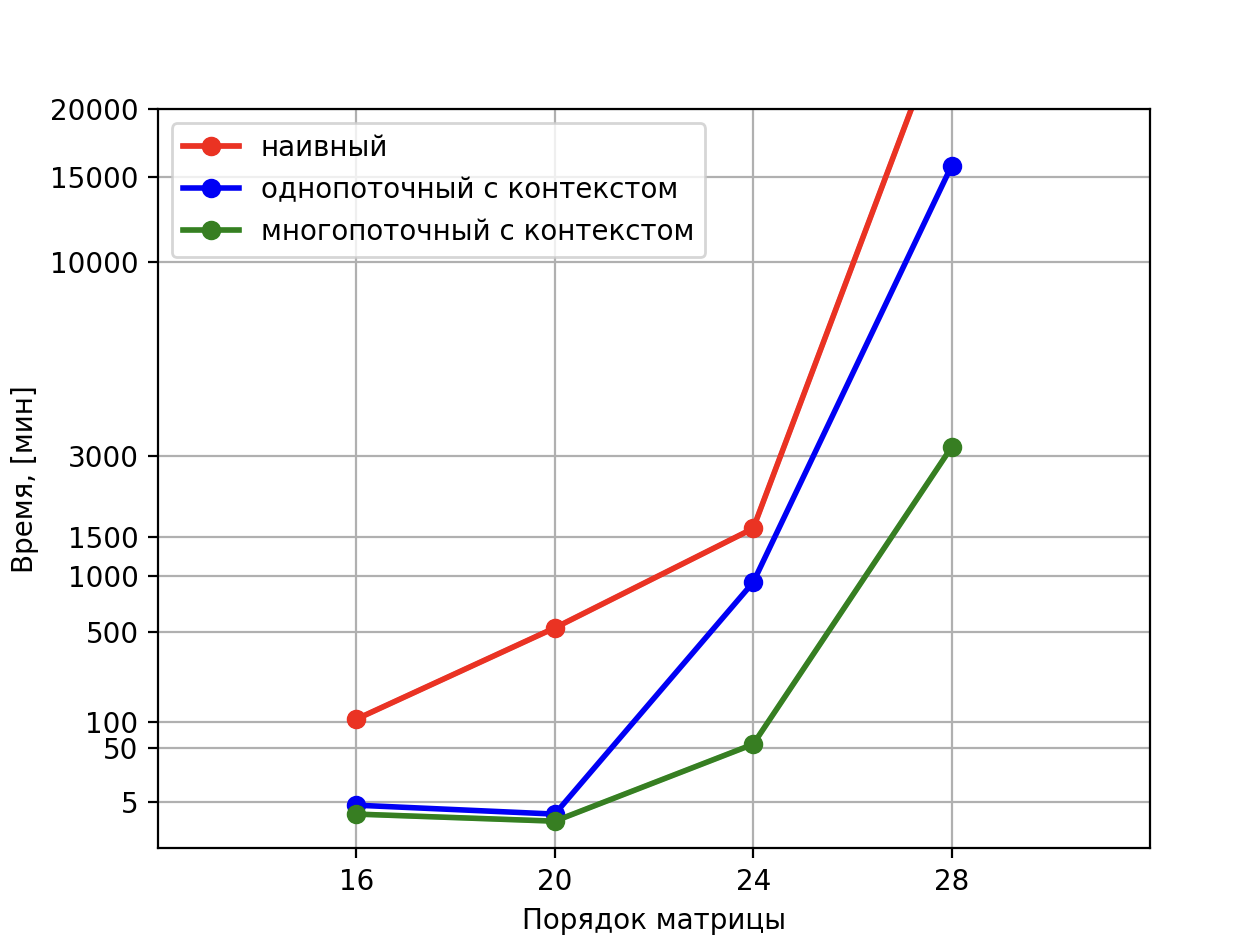
\includegraphics[scale=0.6]{res/img/plot_result.png}
    \caption{График сравнения времени работы различных вариаций алгоритма поиска классов Q-эквивалентности}
    \label{fig:res_plot}
\end{figure}

Можно заметить, что оптимизации дали нам существенный выигрыш по времени работы программы. А также, что алгоритм без оптимизаций работает существенно быстрее заявленной верхней оценки вычислительной сложности, как и говорилось в подразделе \ref{mm_finder_th}.

\nocite{horadam:hma}